\section{Design}\label{sec: Design}
In this section the design and decisions that where made to achieve the laboratory are discussed.

\subsection{ATM machine Part I}\label{subsec: ATM machine Part I}
The software of the previous lab has been split up into two files so that the main logic and main program flow is in the main file and the functions are separated in an atm\_func file. Furthermore a file I/O for login errors was implemented to aid assistance by unusual behavior. The two code listening are shown in Listening \ref{lst: Python code for an ATM Part I} nad \ref{lst: Python functions for an ATM Part I}. A single function is shown in Listening \ref{lst: Python function mainMenu}.

\begin{lstlisting}[style=PythonStyle, language=Python, caption={Python function mainMenu .},label=lst: Python function mainMenu ]
def mainMenue ( ) :
	print ( " Main Menu" )
	print ( "------------------------ \n" )
	print ( " 1 . CHECK BALANCE" )
	print ( " 2 . WITHDRAW CASH" )
	print ( " 3 . DEPOSIT CASH" )
	print ( " 4 . CHANGE PIN" )
	print ( " 5 . EXIT " )
	return 1 # no error 1 , error 0
\end{lstlisting}

The following Listening shows the function call in the main program. That shows how bigger programs in python can be structured sequentially.

\begin{lstlisting}[style=PythonStyle, language=Python, caption={Python function call mainMenu .},label=lst: Python function call mainMenu ]
mainMenue () 
\end{lstlisting}
The following listening shows the error log output file content. This can be easily used to check which errors has been tested and has a message generated to it. The eroor log is continuously appended into a text file and has to be managed manually so far this can be automated with a script as example.
\begin{verbatim}
Thu Oct 25 09:15:45 2018ATM program starts 
Thu Oct 25 09:15:54 2018 User logged in 
Thu Oct 25 09:16:06 2018 Withdraw error
Thu Oct 25 09:16:19 2018 Deposit error
Thu Oct 25 09:16:34 2018 User PIN error
Thu Oct 25 09:27:05 2018 Program Closed
\end{verbatim}

\subsection{ATM machine Part II}\label{subsec: ATM machine Part II}
In this part the program was expended with an receipt function that would log all the transactions of a ongoing section and let the user decide to print it out the end of the session. Figure \ref{fig: Printed receipt} shows how the user can decide after exiting the program if he wishes to print the receipt or not. The python code himself for file I/O used can be examen in closer detail in Listening \ref{lst: Python code for an ATM Part II} and \ref{lst: Python code for an ATM Part II functions}. First a file has to be open this can be done with open(<filename>, mode) and then be accessed with the functions .read() and .write(). 

\begin{figure}[H]
	\centering
	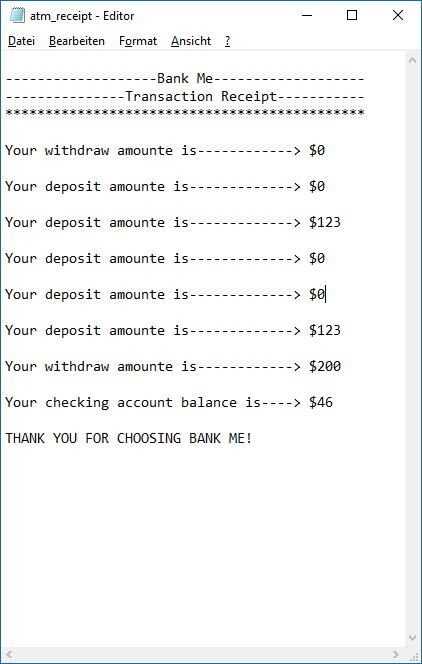
\includegraphics[width=0.5\textwidth]{01_images/printed_receipt.PNG}
	\caption{Printed receipt.}
	\label{fig: Printed receipt}
\end{figure}

\subsection{ATM machine Part II}\label{subsec: ATM machine Part III}

